SQLNet

\item The model was designed to demonstrate that reinforcement learning should be limited in Text2SQL tasks.
\item Until SQLNet, all previous models used reinforcement learning to improve the decoder results when it generated appropriate serializations.
\item In cases where order is irrelevant, SQLNet avoids the seq2seq structure.
\item For making predictions, the model uses a sketch-based approach consisting of a dependency graph that allows previous predictions to be taken into account.
\item To improve the results, the model also incorporates column attention (weights assigned to significant words and phrases in sentences).
\item According to the flowchart below, SQLNet employs three phases to generate SQL queries for WikiSQL tasks.

% add image sqlnet.png
\begin{figure}[htb]
\centering
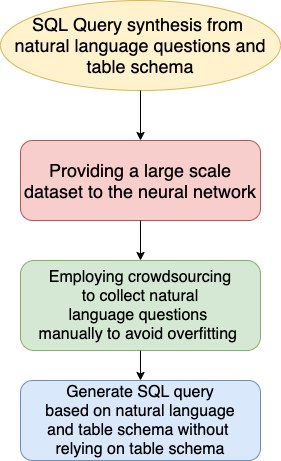
\includegraphics[width=0.8\textwidth]{sqlnet.png}
\caption{SQLNet}
\label{fig:sqlnet}
\end{figure}

Sketch-based query synthesis
The token with the \$ sign represents an empty slot, and the token name represents the type of prediction. Tokens in bold represent SQL keywords such as SELECT, WHERE, etc.
\$AGG can be filled with either an empty token or one of the aggregation operators, such as SUM or MAX. Fill in the \$COLUMN and \$VALUE slots with the column name and substring of the question, respectively. The \$OP slot can be a value between \{=, \}. The notion \(...\)* uses a regular expression to indicate zero or more AND clauses.

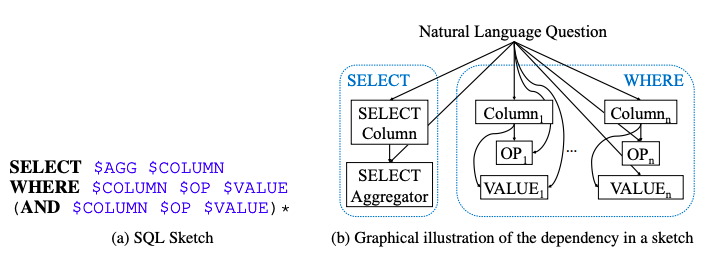
\includegraphics[width=\textwidth]{sketch-based.png}